\documentclass{VUMIFPSmagistrinis}
\usepackage{algorithmicx}
\usepackage{algorithm}
\usepackage{algpseudocode}
\usepackage{amsfonts}
\usepackage{amsmath}
\usepackage{bm}
\usepackage{caption}
\usepackage{color}
\usepackage{float}
\usepackage{graphicx}
\usepackage{listings}
\usepackage{subfig}
\usepackage{wrapfig}


\university{Vilniaus universitetas}
\faculty{Matematikos ir informatikos fakultetas}
\department{Informatikos institutas}
\papertype{Programų sistemų architektūros ir projektavimo laboratorinis darbas}
\title{Architektūriniai požiūriai}
\titleineng{Architectural viewpoints}
\author{Matas Savickis}
\reviewer{}

\supervisor{Rimantas Kybartas, Partn. Prof., Dr.}

\date{Vilnius – \the\year}

\bibliography{bibliografija}

\begin{document}
\maketitle

\tableofcontents
	\section{Sistema}
		Žmonės turi daiktų, kuriuos nori parduoti, tačiau nežino kiek tiksliai jų parduodamas daiktas gali būti vertas.
		Sistema leidžia vartotojams parduoti daiktus aukciono principu.
		Vartotojas įdeda norimą daiktą į aukcioną nustatydamas mažiausią kainą už kurią sutiktų parduoti daiktą, nustato aukciono trukmę ir kiti sistemos parduotojai gali didinti daikto kainą iki nustatyto laiko.
		Sistema suteikia galimybę atsiskaityti už prekes elektroninio banko pervedimais ir kriptovaliutomis.
	\section{Suinteresuoti asmenys}
		\begin{itemize}
			\item{Pirkėjai - vartotojai, kurie naudosis aukcionu siekdami parduoti prekę.}
			\item{Pardavėjai - vartotojai, kurie naudosis aukcionu siekdami nusipirkti prekę.}
			\item{Investuotojai - žmonės, kurie rems projekto įgyvendinimą finansiškai}
			\item{Programuotojai - žmonės, kurie kurs sistemą.}
			\item{Testuotojai - žmonės, kurie testuos sistemą.}
		\end{itemize}
	\section{Požiūrio taškai}
		\section{Konteksto požiūrio taškas}
			\subsection{Sistemos taikymo sritis}
				Vartotojas sistemoje įkelią savo skelbimą, kiti vartotojai dalyvauja aukcione ir didžiausią kainą pasiūlęs vartotojas laimi aukcioną.
				Aukcioną laimėjęs žmogus perveda pinigus arba Bitcoin kripto valiutą į mūsų sistema, tuomet prekės pardavėjas išsiunčia prekę į mūsų biurą patikrinti ar prekė atitinka aprašymą. 
				Biuro darbuotojui patvirtinus, kad prekė atitinka aprašymą sistema perveda pinigus pardavėjui jo pasirinktu būdu.

			\subsection{Konteksto požiūrio taško diagrama}

				\begin{figure}[H]
				\centering
				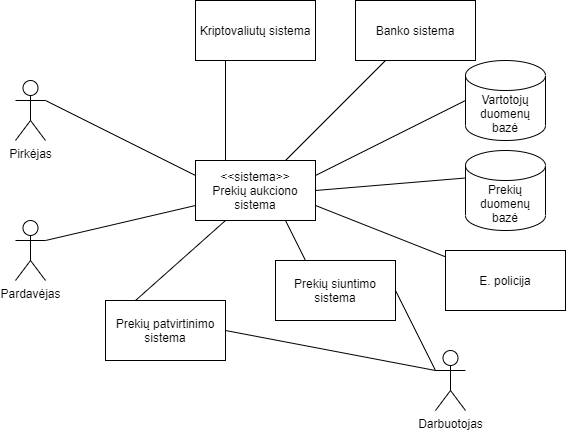
\includegraphics[scale=0.9]{img/context}
				\caption{Aukciono sistemos konteksto požiūrio taško diagrama} % Antraštė įterpiama po paveikslėlio
				\label{img:text}
				\end{figure}
		\section{Funkcinis požiūrio taškas}
		\section{Informacijos požiūrio taškas}
		\section{Lygiagretumo požiūrio taškas}
		\section{Kūrimo požiūrio taškas}
		\section{Diegimo požiūrio taškas}
		\section{Operatyvinis požiūrio taškas}
		


\end{document}
